\subsection{Mathematical Modeling}

\subsubsection{Activation Function: Gaussian Error Linear Unit (GELU)}
Activation functions play a crucial role in introducing non-linearity to the feedforward neural network layers. Following the self-attention mechanism's processing of input data, the results traverse through the feedforward neural network. This network involves linear transformations, and activation functions, such as the Gaussian Error Linear Unit (GELU), are applied element-wise. Activation functions enable the network to grasp and approximate complex, non-linear relationships within the data.

\noindent The Gaussian Error Linear Unit (GELU) stands as an essential activation function within artificial neural networks. Specifically designed to introduce non-linearity to computational processes, GELU offers a seamless approximation to the rectifier linear unit (ReLU) while preserving differentiability.

\noindent Two formulations of the GELU function are commonly used:

\begin{equation}
    \text{GELU}(x) = 0.5x \left(1 + \tanh\left(\frac{\pi}{2} \cdot \left(x + 0.044715x^3\right)\right)\right) \label{eq:gelu}
\end{equation}

\noindent and

\begin{equation}
    \text{GELU}(x) = \frac{1}{2}x \left(1 + \text{erf}\left(\frac{x}{\sqrt{2}}\right)\right) \label{eq:gelu2}
\end{equation}

\noindent Where:
\begin{itemize}
    \item $x$ is the input to the GELU function.
    \item $\text{erf}(z)$ is the error function.
    \item $\pi$ represents the mathematical constant pi.
    \item $\sqrt{2}$ is the square root of 2.
\end{itemize}

\noindent The GELU activation function is often used in neural network architectures due to its smoothness and differentiability properties, making it suitable for gradient-based optimization during training.

\noindent Additionally, consider the mathematical expression:
\begin{equation}
    P(X = c) \label{eq:probability}
\end{equation}

\noindent where $X$ represents a random variable and $c$ is a constant value. This expression is used to represent the probability that the random variable $X$ takes on the value $c$.

\noindent When no activation function is used in a neural network, the model essentially reduces to a linear regression or a linear transformation. Consequently, the entire neural network collapses into a single linear transformation, regardless of the number of layers. This severely limits the expressive power of the network, as it can only learn linear relationships in the data.

\noindent Compared to Rectified Linear Unit (ReLU) and Exponential Linear Unit (ELU), the Gaussian Error Linear Unit (GELU) activation function stands out for its smoothness, handling of negative inputs, and ability to capture complex patterns. ReLU sets all negative values to zero during the forward pass, which can lead to "dead neurons" that never activate and do not contribute to learning. This can result in a loss of information and slower convergence during training. Whereas, ELU largely suffers from vanishing gradient problem.

\begin{figure}[htbp]
    \centering
    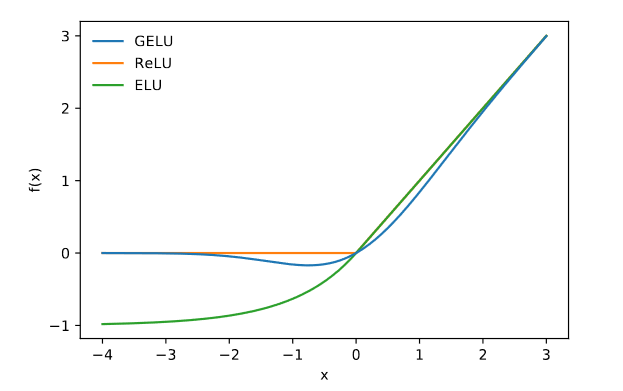
\includegraphics[width=6in]{img/gelu vs relu.png}
    \caption{{GeLU vs ReLU vs ELU graph}}
\end{figure}

\noindent Compared to Rectified Linear Unit (ReLU) and Exponential Linear Unit (ELU), the Gaussian Error Linear Unit (GELU) activation function stands out for its smoothness, handling of negative inputs, and ability to capture complex patterns. ReLU sets all negative values to zero during the forward pass, which can lead to "dead neurons" that never activate and do not contribute to learning. This can result in a loss of information and slower convergence during training. Whereas, ELU largely suffers from vanishing gradient problem.

\subsubsection{Loss Function}
The loss function employed in the Vision Transformer (ViT) model is a critical component for training the network and optimizing its performance in image classification tasks. The ViT loss function is designed to measure the disparity between the predicted class probabilities and the ground truth labels.

\paragraph{Cross-Entropy Loss :}
The primary loss utilized in ViT is the Cross-Entropy Loss, also known as categorical cross-entropy. It quantifies the difference between the predicted probability distribution (produced by the softmax activation) and the true distribution of class labels.

\noindent Mathematically, the Cross-Entropy Loss for a single training example is defined as:

\begin{equation}
    L(y, \hat{y}) = -\sum_i y_i \cdot \log(\hat{y}_i) \label{eq:loss_function}
\end{equation}

\noindent where:
\begin{align*}
    y       & \text{ is the ground truth label vector,}                 \\
    \hat{y} & \text{ is the predicted probability distribution vector,} \\
    i       & \text{ iterates over all classes.}
\end{align*}

\subsubsection{Bilinear Interpolation }
Bilinear interpolation is a widely used technique in image processing for estimating pixel values at non-integer coordinates within an image. This method is particularly valuable when scaling or resizing images, offering a smoother transition between neighboring pixels compared to simpler interpolation methods ensuring a smoother and visually appealing transition between pixel values, contributing to improved image quality in various computer graphics and computer vision applications.

\noindent \subparagraph{Steps}
\begin{enumerate}
    \item \textbf{Identify Neighboring Pixels:}Given a non-integer coordinate (x, y), locate the four nearest pixels in the image: (x1, y1), (x1, y2), (x2, y1), and (x2, y2), defining a rectangular region

    \item \textbf{Calculate Interpolation Weights:} Compute the horizontal (u) and vertical (v) interpolation weights based on the fractional part of the coordinates (x, y).
          \begin{align}
              u & = x - x_1 \label{eq:u_equation} \\
              v & = y - y_1 \label{eq:v_equation}
          \end{align}


    \item \textbf{Perform Interpolation:} Interpolate along the vertical direction to obtain the interpolated value:
          \begin{align}
              I_{\text{interpolated}} & = (1 - v) \cdot I_{\text{top}} + v \cdot I_{\text{bottom}} \label{eq:interpolated_equation}
          \end{align}


          \text{where:}
          \begin{align}
              I_{\text{top}}    & = (1 - u) \cdot I(x_1, y_1) + u \cdot I(x_2, y_1) \label{eq:itop_equation}    \\
              I_{\text{bottom}} & = (1 - u) \cdot I(x_1, y_2) + u \cdot I(x_2, y_2) \label{eq:ibottom_equation}
          \end{align}


\end{enumerate}
\subsubsection{Layer Normalization}
The Layer Normalization is applied independently to each position (or patch) in the input sequence.Layer Normalization is very similar to Batch normalization but layer normalization is favored because it works independently on each patch of the image sequence, aligning well with ViT's sequential processing.

\noindent Given an input tensor $x$ at a particular position, the Layer Normalization is computed using the formula:

\begin{equation}
    \text{LayerNorm}(x) = \frac{x - \text{mean}(x)}{\sqrt{\text{var}(x) + \epsilon}} \cdot \gamma + \beta \label{eq:layer_norm}
\end{equation}

\noindent Here, $\text{mean}(x)$ and $\text{var}(x)$ represent the mean and variance of the input $x$ at that position, and $\gamma$ and $\beta$ are learnable parameters. $\epsilon$ is a small constant for numerical stability.

\noindent \textbf{Importance:}
Layer Normalization is crucial for stabilizing training by normalizing the activations at each position. It helps mitigate change in the distribution of the input during training, making the model less sensitive to changes in input distribution. This normalization facilitates more stable and efficient training, enabling the model to better capture complex hierarchical features in image data.

\subsubsection{Positional Encoding}
Positional encoding is used Vision Transformer to provide information about the position of tokens in a sequence. Since transformers don't inherently understand the order of tokens, positional encoding helps inject spatial information into the input data.

\noindent Formula for 1D positional encoding for a token at position $pos$ in a sequence of length $L$ with embedding dimension $d$:

\begin{equation}
    \text{PE}(pos, 2i) = \sin\left(\frac{pos}{10000^{2i/d}}\right) \label{eq:pos_encoding_sin}
\end{equation}

\begin{equation}
    \text{PE}(pos, 2i+1) = \cos\left(\frac{pos}{10000^{2i/d}}\right) \label{eq:pos_encoding_cos}
\end{equation}


\noindent Here, $pos$ is the position, $i$ is the dimension, and $d$ is the embedding dimension. The positional encoding values are added to the original embeddings of the tokens.

\noindent In essence, the formula generates unique sinusoidal patterns for each position and dimension, enabling the model to distinguish the order of tokens in the sequence. This helps transformers effectively process sequential data, such as text or images divided into patches.

\subsubsection{Softmax Score}
The softmax function is used to convert a vector of real numbers into a probability distribution. In the context of machine learning and neural networks, it is often applied to the raw scores or logits produced by the model. The softmax function ensures that the values in the resulting vector are between 0 and 1 and sum to 1. It's commonly used in the output layer of a classification model to obtain probabilities for each class.

\noindent Given an input vector \(z\) with \(K\) elements, the softmax function is calculated as follows:
\begin{equation}
    \text{Softmax}(z)_i = \frac{e^{z_i}}{\sum_{j=1}^{K} e^{z_j}} \label{eq:softmax}
\end{equation}


\noindent Here, \(\text{Softmax}(z)_i\) represents the \(i\)-th element of the resulting softmax vector. \(e\) is the base of the natural logarithm (Euler's number). The numerator is the exponentiation of the \(i\)-th element of \(z\), and the denominator is the sum of the exponentiations of all elements in \(z\).

\noindent The softmax operation essentially transforms the input vector into a probability distribution, making it suitable for tasks like multiclass classification where the goal is to assign probabilities to different classes.

\subsubsection{Adam Optimizer}

\noindent The Adam optimizer, short for Adaptive Moment Estimation, combines the advantages of adaptive learning rates, momentum optimization, and the Root Mean Square Propagation (RMSProp) algorithm. Adam is known for its efficiency, stability, and adaptability across a variety of neural network architectures and datasets.

\noindent Adam excels in handling large datasets with varying or sparse gradients. It dynamically adjusts learning rates for each parameter, enhancing adaptability during training. By integrating momentum and RMSProp techniques, Adam accelerates convergence and prevents local minima.

\noindent The Adam optimizer updates model parameters based on the following mathematical expressions:

\begin{enumerate}
    \item \textbf{Initialization:}
          \begin{equation}
              m_0 = 0, \quad v_0 = 0
          \end{equation}

    \item \textbf{Moments computation (for obtaining minimum approximation)}
          \begin{align}
              m_t & = \beta_1 \cdot m_{t-1} + (1 - \beta_1) \cdot g_t   \\
              v_t & = \beta_2 \cdot v_{t-1} + (1 - \beta_2) \cdot g_t^2
          \end{align}

    \item \textbf{Bias Correction:}
          \begin{align}
              \hat{m}_t & = \frac{m_t}{1 - \beta_1^t} \\
              \hat{v}_t & = \frac{v_t}{1 - \beta_2^t}
          \end{align}

    \item \textbf{Update Parameters:}
          \begin{equation}
              \theta_{t+1} = \theta_t - \frac{\eta}{\sqrt{\hat{v}_t} + \epsilon} \cdot \hat{m}_t
          \end{equation}
\end{enumerate}

Where:
\begin{itemize}
    \item \( \eta \) is the learning rate.
    \item \( \beta_1 \) and \( \beta_2 \) control the exponential decay rates for the moment estimates.
    \item \( \epsilon \) is a small constant to prevent division by zero.
\end{itemize}

\noindent These equations describe the adaptive learning rate mechanism and the combination of momentum and RMSProp, for Adams Optimizer.





